% !TeX document-id = {c68f4be8-c497-43e0-82df-e9ebfbea9577}
% !TeX TXS-program:pdflatex = pdflatex -synctex=1 -interaction=nonstopmode --shell-escape %.tex
% новая команда \RNumb для вывода римских цифр
\documentclass[a4paper,12pt]{article}
\usepackage{amssymb}
\usepackage{amsmath}
\usepackage{amsthm} 
\usepackage{caption}
\usepackage{misccorr}
\usepackage[noadjust]{cite}
\usepackage{cmap} 
\usepackage[utf8]{inputenc}
\usepackage[T2A]{fontenc}
\usepackage[english, russian]{babel}
\usepackage{graphics}
\usepackage{graphicx}
\usepackage{textcomp}
\usepackage{verbatim}
\usepackage{makeidx}
\usepackage{geometry}
\usepackage{float}
\usepackage{bm}
\usepackage{esint}
\usepackage{mathtools}
\usepackage{graphicx}
\usepackage{listings}
\usepackage{courier}
\usepackage{multirow}
\usepackage{graphicx}

\lstset{basicstyle=\fontsize{10}{10}\selectfont,breaklines=true}

\newcommand{\specchapter}[1]{\chapter*{#1}\addcontentsline{toc}{chapter}{#1}}
\newcommand{\specsection}[1]{\section*{#1}\addcontentsline{toc}{section}{#1}}
\newcommand{\specsubsection}[1]{\subsection*{#1}\addcontentsline{toc}{subsection}{#1}}
\newcommand{\RNumb}[1]{\uppercase\expandafter{\romannumeral #1\relax}}
\newcommand{\jj}{\righthyphenmin=20 \justifying}


% геометрия
\geometry{pdftex, left = 2cm, right = 2cm, top = 2.5cm, bottom = 2.5cm}

\setcounter{tocdepth}{4} % фикс переноса 
\righthyphenmin = 2
\tolerance = 2048

\begin{document}
\thispagestyle{empty}

\noindent \begin{minipage}{0.15\textwidth}
	
\includegraphics[width=\linewidth]{b_logo}
\end{minipage}
\noindent\begin{minipage}{0.9\textwidth}\centering
	\textbf{Министерство науки и высшего образования Российской Федерации}\\
	\textbf{Федеральное государственное бюджетное образовательное учреждение высшего образования}\\
	\textbf{«Московский государственный технический университет имени Н.Э.~Баумана}\\
	\textbf{(национальный исследовательский университет)»}\\
	\textbf{(МГТУ им. Н.Э.~Баумана)}
\end{minipage}

\noindent\rule{18cm}{3pt}
\newline\newline
\noindent ФАКУЛЬТЕТ $\underline{\text{«Информатика и системы управления»}}$ \newline\newline
\noindent КАФЕДРА $\underline{\text{«Компьютерные системы и сети»}}$\newline\newline
\noindent НАПРАВЛЕНИЕ ПОДГОТОВКИ $\underline{\text{«09.03.04 Программная инженерия»}}$\newline\newline\newline\newline\newline


\begin{center}
	\noindent\begin{minipage}{1.3\textwidth}\centering
	\Large\textbf{  ОТЧЕТ }\newline
	\textbf{по лабораторной работе №2}\newline\newline
	\end{minipage}
\end{center}

\noindent\textbf{Название:} $\underline{\text{Исследование дешифраторов}}$\newline\newline
\noindent\textbf{Дисциплина:} $\underline{\text{Архитектура ЭВМ}}$\newline\newline\newline\newline\newline

\begin{center}
	\begin{tabular}{ccccc}
		Студент: & $\underline{\text{ИУ7-43Б}}$ & $\underline{\text{~~~~~~~~~~~}}$ & $\underline{\text{02.04.2020}}$ & $\underline{\text{А. В. Романов}}$ \\
		 & \footnotesize группа & \footnotesize подпись & \footnotesize дата  & \footnotesize (И. О. Фамилия) \\
		  &  &  &  & \\
		Преподаватель: & \textbf{} & $\underline{\text{~~~~~~~~~~~}}$ & $\underline{\text{~~~~~~~~~~~~}}$ & $\underline{\text{А. Ю. Попов}}$ \\
		&  & \footnotesize подпись & \footnotesize дата  & \footnotesize (И. О. Фамилия) \\
	\end{tabular}
\end{center}


\begin{center}
	\vfill
	Москва~---~\the\year
~г.
\end{center}
\clearpage

\section{Цель работы} Изучение принципов построения методов синтеза дешифраторов; макетирование и экспериментальное исследования дешифраторов

\section{Линейный двухвходовый дешифратор}

\begin{center}
	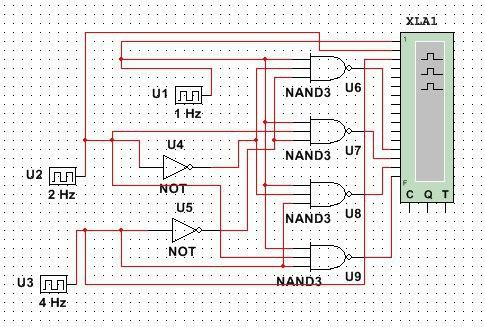
\includegraphics[scale=1.1]{../screens/1.jpg} \newline\newline 
	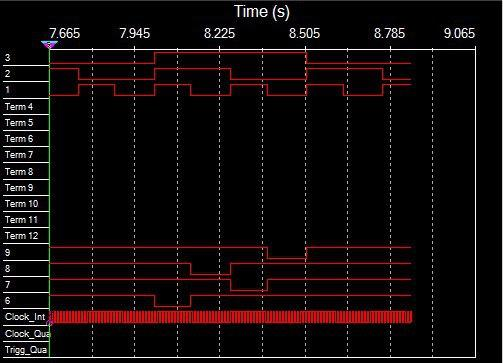
\includegraphics[scale=1.1]{../screens/1_2.jpg} \newline\newline 
	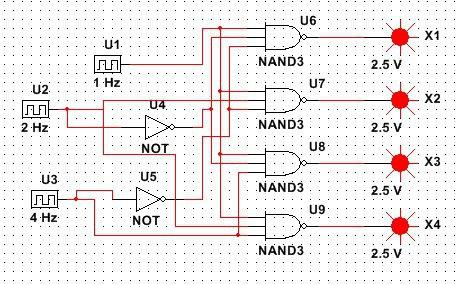
\includegraphics[scale=1.1]{../screens/1_3.jpg} \newline
	
	Таблица переходов:
	\begin{center}
		\begin{tabular}{ | l | l | l | l | l | l | l | p{1cm} |}
			\hline
			$E$ & $A_{1}$ & $A_{2}$ & $F_{1}$ & $F_{2} $ & $F_{3}$ & $F_{4}$ \\ \hline
			0 & * & * & 1 & 1 & 1 & 1\\ \hline
			1 & 0 & 0 & 0 & 1 & 1 & 1\\ \hline
			
			1 & 0 & 1 & 1 & 0 & 1 & 1\\ \hline 
			1 & 1 & 0 & 1 & 1 & 0 & 1\\ \hline
			
			1 & 1 & 1 & 1 & 1 & 1 & 0 \\ 
			\hline
		\end{tabular}
	\end{center}
\end{center}

\noindent Так как мы моделируем в компьютере (не в реальной жизни), устранять гонки сигналов не обязательно. Чтобы их не было в реально жизни, нужно чтобы стобирующий сигнал не был равен единице во время переключения сигналов. Тут получается среднее время задержки равно сумме средних времен сигнала через НЕ и И-НЕ.\newline

\noindent Файлы: 1.ms12 и 2.ms12

\clearpage
\section{Дешифратор ИС К155ИД4}

\begin{center}
	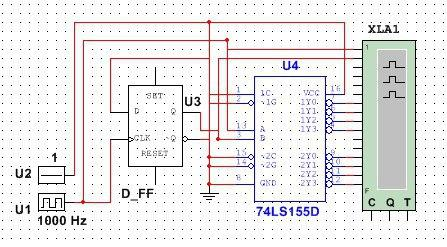
\includegraphics[scale=1.3]{../screens/2_1.jpg} \newline\newline\newline\newline
	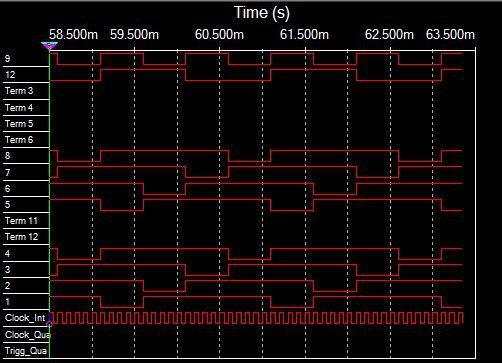
\includegraphics[scale=1.3]{../screens/2_2.jpg} \newline\newline
	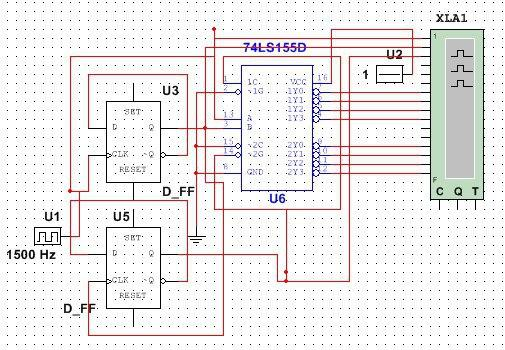
\includegraphics[scale=0.9]{../screens/3_1.jpg} \newline\newline
	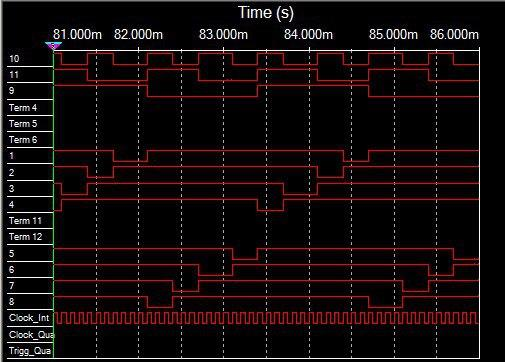
\includegraphics[scale=0.9]{../screens/3_2.jpg} \newline
	
	Таблица переходов: 
	
	\begin{center}
		\begin{tabular}{ | l | l | l | l | l | l | l | l | l | l | l | p{1cm} |}
			\hline
			$A_{1}$ & $A_{2}$ & $A_{3}$ & $F_{1}$ & $F_{2}$ & $F_{3}$ & $F_{4}$ & $F_{5}$ & $F_{6}$ & $F_{7}$ & $F_{8}$ \\ \hline
			0 & 0 & 0 & 0 & 1 & 1 & 1 & 1 & 1 & 1 & 1 \\ \hline
			0 & 0 & 1 & 1 & 0 & 1 & 1 & 1 & 1 & 1 & 1 \\ \hline 
			0 & 1 & 0 & 1 & 1 & 0 & 1 & 1 & 1 & 1 & 1 \\ \hline
			0 & 1 & 1 & 1 & 1 & 1 & 0 & 1 & 1 & 1 & 1 \\ \hline
			1 & 0 & 0 & 1 & 1 & 1 & 1 & 0 & 1 & 1 & 1 \\ \hline
			1 & 0 & 1 & 1 & 1 & 1 & 1 & 1 & 0 & 1 & 1 \\ \hline
			1 & 1 & 0 & 1 & 1 & 1 & 1 & 1 & 1 & 0 & 1 \\ \hline
			1 & 1 & 1 & 1 & 1 & 1 & 1 & 1 & 1 & 1 & 0 \\
			\hline
		\end{tabular}
	\end{center}
\end{center}

\noindent Файлы: 3.ms12 и 4.ms12

\section{Исследование дешифраторов ИС КР531ИД14}


\begin{center}
	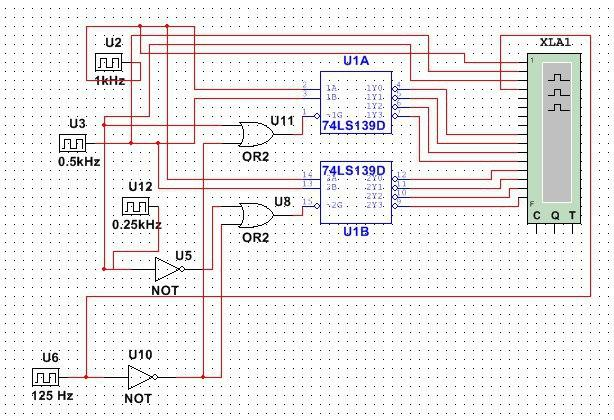
\includegraphics[scale=1]{../screens/4_1.jpg} \newline\newline 
	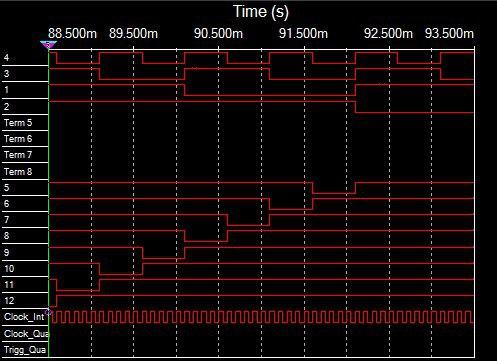
\includegraphics[scale=1]{../screens/4_2.jpg} \newline
\end{center}

\noindent Файл: 5.ms12

\clearpage
\section{Трехвходовый дешифратор 533ИД7}

\begin{center}
	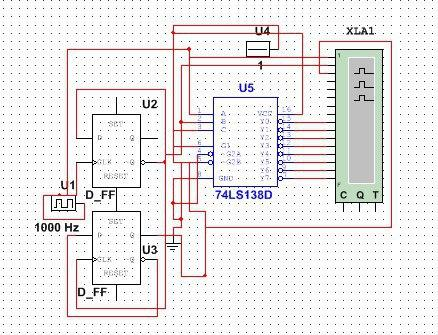
\includegraphics[scale=1]{../screens/5_1.jpg} \newline\newline
	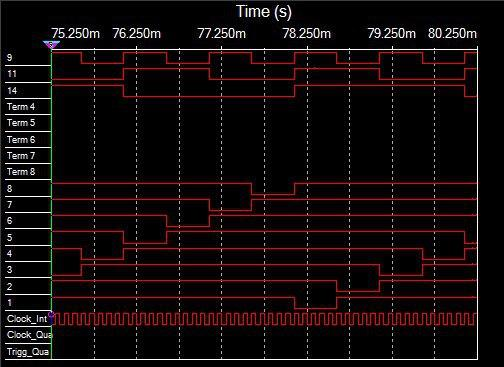
\includegraphics[scale=1]{../screens/5_2.jpg} \newline
\end{center}

\noindent Файл: 6.ms12

\section{Вывод}

\noindent При выполнении этой лабораторной работы я изучил принципы построения и методы синтеза дешифраторов, при этом эксперементально изучив дешифраторы.

\section{Контрольные вопросы}

\noindent\textbf{1.} Что называется дешифратором?\newline

\noindent\textbf{Дешифратор} -- комбинационный узел с $n$ входами и $N$ выходами, преобразующий каждый набор двоичных сигналов в активный сигнал на выходе, соответствующий этому набору.\newline

\noindent\textbf{2.} Какой дешифратор называется полным (неполным)? \newline

\noindent Дешифратор, имеющий $2n$ выходов, называется полным, при меньшем числе выходов -- неполным.
\newline

\noindent\textbf{3.} Определите закон функционирования дешифратора аналитически и таблично.\newline

\noindent Функционирование дешифратора $DC$ $n-N$ определяется таблицей истинности:

\begin{center}
	\begin{tabular}{ | l | l | l | l | l | l | l | l | l | l | l | l | l | p{1cm} |}
			\hline
			 \multicolumn{7}{|c|}{Входы} &  \multicolumn{6}{|c|}{Выходы} \\ \hline
			$EN$ & $A_{n - 1}$ & $A_{n - 2}$ & $A_{n - 3}$ & ... & $A_{1}$ & $A_{0} $ & $F_{0} $ & $F_{1}$ & $F_{2}$ & ... & $F_{N - 2}$ & $F_{N - 1}$ \\ \hline
			
			0 & x & x & x & ... & x & x & 0 & 0 & 0 & ... & 0 & 0 \\ \hline
			1 & 0 & 0 & 0 & ... & 0 & 0 & 1 & 0 & 0 & ... & 0 & 0 \\ \hline
			1 & 0 & 0 & 0 & ... & 0 & 1 & 0 & 1 & 0 & ... & 0 & 0 \\ \hline
			1 & 0 & 0 & 0 & ... & 1 & 0 & 0 & 0 & 1 & ... & 0 & 0 \\ \hline
			
			. & . & . & . & ... & . & . & . & . & . & ... & . & . \\ \hline
			. & . & . & . & ... & . & . & . & . & . & ... & . & . \\ \hline
			. & . & . & . & ... & . & . & . & . & . & ... & . & . \\ \hline
			
			1 & 1 & 1 & 1 & ... & 1 & 0 & 0 & 0 & 0 & ... & 1 & 0 \\ \hline
			1 & 1 & 1 & 1 & ... & 0 & 1 & 0 & 0 & 0 & ... & 0 & 1 \\ 
			\hline
	\end{tabular}
\end{center}

\noindent Аналитически описать дешифратор можно совокупностью логических функций в СДНФ:
$$ F_{0} = EN \cdot \overline{A}_{n - 1}  \cdot \overline{A}_{n - 2}  \cdot ... \cdot \overline{A}_{i} \cdot \overline{A}_{1} \cdot \overline{A}_{0}, $$
$$ F_{1} = EN \cdot \overline{A}_{n - 1}  \cdot \overline{A}_{n - 2}  \cdot ... \cdot \overline{A}_{i} \cdot \overline{A}_{1} \cdot A_{0}, $$
$$ F_{2} = EN \cdot \overline{A}_{n - 1}  \cdot \overline{A}_{n - 2}  \cdot ... \cdot \overline{A}_{i} \cdot A_{1} \cdot \overline{A}_{0}, $$
$$. . . . . . . . . . . . . . . . . . . . . . . . . . . . . . . . . . . . . . . . . . . . . . . . . . . . . . . . . . . . . . .$$
$$ F_{N - 2} = EN \cdot A_{n - 1}  \cdot A_{n - 2}  \cdot ... \cdot A_{i} \cdot A_{1} \cdot \overline{A}_{0}, $$
$$ F_{N - 1} = EN \cdot A_{n - 1}  \cdot A_{n - 2}  \cdot ... \cdot A_{i} \cdot A_{1} \cdot A_{0}, $$

\clearpage
\noindent\textbf{4.} Поясните основные способы построения дешифраторов.\newline

\noindent Линейный дешифратор строится в соответствии с системой, представленной в предыдущем вопросе, и представляет собой $2^n$ конъюнкторов или логических элементов ИЛИ-НЕ с $n$-входами каждый при отсутствии стробирования и с $n + 1$ входами - при его наличии. \newline
Пирамидальный дешифратор строится на основе последовательной (каскадной) реализации выходных функций. \textit{На первом этапе} реализуются конъюнкции двух переменных. \textit{На втором} – все конъюнкции трех переменных путем логического умножения каждой ранее полученной конъюнкции двух переменных на переменную.. Таким образом, на каждом следующем этапе получают вдвое больше конъюнкции, чем на предыдущем. Пирамидальные дешифраторы независимо от числа их входов строятся на основе только двухвходовых конъюнкторов.
\newline

\noindent\textbf{5.} Что называется гонками и как устраняются ложные сигналы, вызванные гонками?\newline

\noindent Вследствие переходных процессов и временных задержек сигналов в цепях логических элементов могут возникнуть так называемые гонки, приводящие к появлению ложных сигналов на выходах схемы. Основным средством, позволяющим исключить гонки, является стробирование(выделение из информационного сигнала той части, которая  свободна от искажений, вызываемых гонками). Стробирующий сигнал на этом входе не должен быть активным во время переходных процессов в дешифраторе.
\newline

\noindent\textbf{6.} Каковы способы наращивания дешифраторов по количеству входов и выходов и как они реализуются схемотехнически?\newline

\noindent Пусть для построения сложного дешифратора $DC$ $n-N$ используются простые дешифраторы $DC$ $n_{1} - N_{1}$, причем $n_{1} << n$, следовательно и $N_{1} << N$.\newline

\textbf{1. }Число каскадов равно $К = \frac{n}{n1}$. Если К – целое число, то во всех каскадах используются полные дешифраторы $DC$ $n_{1}-N_{1}$. Если $К$ – правильная или смешанная дробь, то во входном каскаде используется неполный дешифратор $DC$ $n_{1} - N_{1}$.\newline

\textbf{2. }Количество простых дешифраторов $DC$ $n_{1} - N_{1}$ в выходном каскаде равно $\frac{N}{N_{1}}$, в предвыходном - $\frac{N}{N_{1}^2}$ , в предпредвыходном - $\frac{N}{N_{1}^3}$ и т.д.; во входном каскаде - $\frac{N}{N_{1}}$. Если $\frac{N}{N_{1}}$ – правильная дробь, то это означает, что во входном каскаде используется неполный простой дешифратор.\newline

\textbf{3. }В выходном каскаде дешифрируются n1 младших разрядов адреса сложного дешифратора, в предвыходном – следующие n1 младших разрядов адреса сложного дешифратора и т.д. Во входном каскаде дешифрируется полная или неполная группа старших разрядов адреса. Поэтому $n_{1}$ младших разрядов адреса сложного дешифратора подаются параллельно на адресные входы всех дешифраторов выходного каскада, следующие $n_{1}$ младших разрядов адреса – на адресные входы всех дешифраторов предвыходного каскада и т.д.; группа старших разрядов адреса подается на адресные входы дешифратора.\newline

\textbf{4. }Выходы дешифраторов предвыходного каскада соединяются с входами разрешения простых дешифраторов выходного каскада, выходы дешифраторов предпредвыходного каскада – с входами разрешения простых дешифраторов предвыходного каскада и тд.


\end{document}